\documentclass[tikz, border=10pt]{standalone}
\usepackage{xcolor}
\usetikzlibrary{calc,arrows.meta,decorations.markings}

% Define path colors matching the PHO visual style
\definecolor{pathBlue}{RGB}{40, 70, 150}
\definecolor{pathOrange}{RGB}{230, 130, 40}
\definecolor{pathGreen}{RGB}{60, 140, 70}

\begin{document}
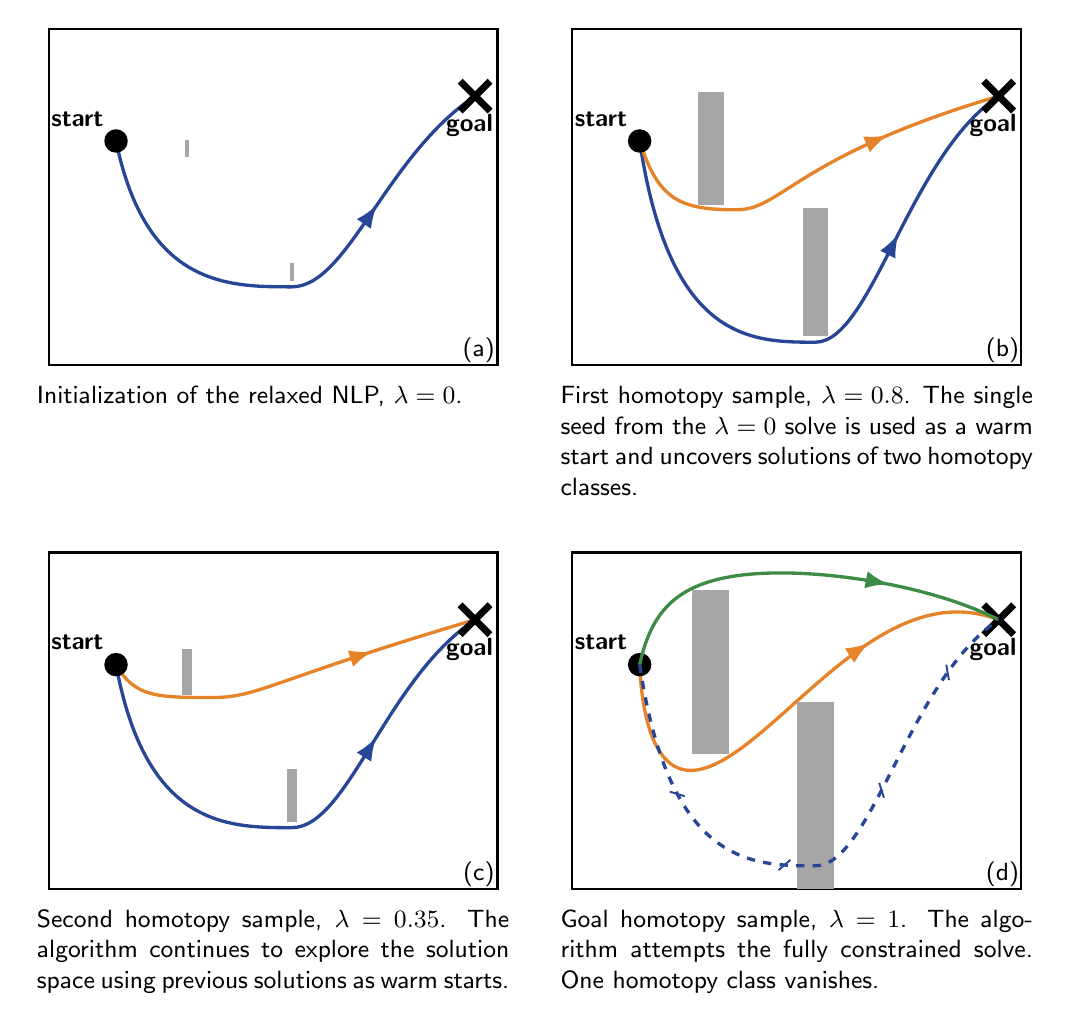
\begin{tikzpicture}[
    scale=0.95,
    path line/.style={
        very thick,
        postaction={decorate},
        decoration={markings, mark=at position 0.72 with {\arrow{Latex}}}
    },
    invalid path/.style={
        very thick,
        dashed,
        postaction={decorate},
        decoration={
            markings,
            mark=at position 0.22 with {\draw[solid, line width=0.7pt] (-2pt,-2pt) -- (2pt,2pt);},
            mark=at position 0.44 with {\draw[solid, line width=0.7pt] (-2pt,-2pt) -- (2pt,2pt);},
            mark=at position 0.66 with {\draw[solid, line width=0.7pt] (-2pt,-2pt) -- (2pt,2pt);},
            mark=at position 0.88 with {\draw[solid, line width=0.7pt] (-2pt,-2pt) -- (2pt,2pt);}
        }
    },
    obstacle/.style={fill=black!35, draw=none},
    label font/.style={font=\sffamily\bfseries\small}
]

% Reusable environment copied from the RRT demonstration.
\def\drawEnvironment#1#2#3#4{
    \draw[thick] (0,0) rectangle (6,4.5);
    \node[font=\sffamily\small] at (5.75, 0.2) {(#4)};
    \pgfmathsetmacro{\topHalfWidth}{0.25*#2}
    \pgfmathsetmacro{\topHalfHeight}{1.1*#2}
    \pgfmathsetmacro{\bottomHalfWidth}{0.25*#3}
    \pgfmathsetmacro{\bottomHalfHeight}{1.25*#3}
    \fill[obstacle]
        ({1.85-\topHalfWidth},{2.9-\topHalfHeight})
        rectangle
        ({1.85+\topHalfWidth},{2.9+\topHalfHeight});
    \fill[obstacle]
        ({3.25-\bottomHalfWidth},{1.25-\bottomHalfHeight})
        rectangle
        ({3.25+\bottomHalfWidth},{1.25+\bottomHalfHeight});
    \coordinate (S) at (0.9,3.0);
    \coordinate (G) at (5.7,3.6);
    \node[circle, fill=black, inner sep=3pt] at (S) {};
    \node[label font, left=1pt, yshift=8pt] at (S) {start};
    \draw[line width=2.5pt] ($(G)+(-0.2,-0.2)$) -- ($(G)+(0.2,0.2)$);
    \draw[line width=2.5pt] ($(G)+(-0.2,0.2)$) -- ($(G)+(0.2,-0.2)$);
    \node[label font, below=3pt, xshift=-2pt] at (G) {goal};
    \node[anchor=north, align=justify, text width=6cm, font=\sffamily\small] at (3,-0.15) {#1};
}

% Panel A: a relaxed seed may cross the obstacles.
\begin{scope}[shift={(0,7.0)}]
    \draw[path line, pathBlue] (0.9,3.0) .. controls (1.3,1.05) and (2.4,1.05) .. (3.25,1.05) .. controls (4.0,1.05) and (4.5,2.8) .. (5.7,3.6);
    \drawEnvironment{Initialization of the relaxed NLP, $\lambda=0$.}{0.10}{0.10}{a}
\end{scope}

% Panel B: the first constrained solve discovers the upper route.
\begin{scope}[shift={(7,7.0)}]
    \draw[path line, pathBlue] (0.9,3.0) .. controls (1.3,0.31) and (2.4,0.31) .. (3.25,0.31) .. controls (4.0,0.31) and (4.5,2.8) .. (5.7,3.6);
    \draw[path line, pathOrange] (0.9,3.0) .. controls (1.15,2.2) and (1.45,2.08) .. (2.2,2.08) .. controls (2.8,2.08) and (3.0,2.8) .. (5.7,3.6);
    \drawEnvironment{First homotopy sample, $\lambda=0.8$. The single seed from the $\lambda=0$ solve is used as a warm start and uncovers
    solutions of two homotopy classes.}{0.685}{0.685}{b}
\end{scope}

% Panel C: the second sample finds the route through the central passage.
\begin{scope}[shift={(0,0)}]
    \draw[path line, pathBlue] (0.9,3.0) .. controls (1.3,0.82) and (2.4,0.82) .. (3.25,0.82) .. controls (4.0,0.82) and (4.5,2.8) .. (5.7,3.6);
    \draw[path line, pathOrange] (0.9,3.0) .. controls (1.15,2.56) and (1.45,2.56) .. (2.2,2.56) .. controls (2.8,2.56) and (3.0,2.8) .. (5.7,3.6);
    \drawEnvironment{Second homotopy sample, $\lambda=0.35$. The algorithm continues to explore the solution space using previous solutions as warm starts.}{0.28}{0.28}{c}
\end{scope}

% Panel D: both feasible homotopy classes are available at the goal problem.
\begin{scope}[shift={(7,0)}]
    \draw[path line, pathOrange]
        plot[domain=0:1, samples=100]
        ({(1-\x)^4*0.9 + 4*(1-\x)^3*\x*1.0 + 6*(1-\x)^2*\x^2*2.2 + 4*(1-\x)*\x^3*3.6 + \x^4*5.7},
         {(1-\x)^4*3.0 + 4*(1-\x)^3*\x*0.75 + 6*(1-\x)^2*\x^2*0.75 + 4*(1-\x)*\x^3*4.4 + \x^4*3.6});
    \drawEnvironment{Goal homotopy sample, $\lambda=1$. The algorithm attempts the fully constrained solve. One homotopy class vanishes.}{1.0}{1.0}{d}
        \draw[path line, pathGreen]
            plot[domain=0:1, samples=100]
            ({(1-\x)^4*0.9 + 4*(1-\x)^3*\x*1.2 + 6*(1-\x)^2*\x^2*2.0 + 4*(1-\x)*\x^3*4.2 + \x^4*5.7},
             {(1-\x)^4*3.0 + 4*(1-\x)^3*\x*4.35 + 6*(1-\x)^2*\x^2*4.35 + 4*(1-\x)*\x^3*4.35 + \x^4*3.6});
    \draw[invalid path, pathBlue] (0.9,3.0) .. controls (1.3,0.31) and (2.4,0.31) .. (3.25,0.31) .. controls (4.0,0.31) and (4.5,2.8) .. (5.7,3.6);
\end{scope}

\end{tikzpicture}
\end{document}